\chapter{运行时调度可变的沙箱机制实现}\label{chap:control_zone}

\section{概述}

% 介绍 Control Zone 的概念

现代服务器上有丰富的计算资源,能够支持大量应用进行混部,相关研究表明,粗略地将应用分为LC与BE忽略了其他混部的可能。细分应用能够挖掘更多的混部可能,但是当前无论是基于资源划分还是任务调度的相关研究,都不能保证在任何混部场景中,都能有效地对目标应用的QoS进行保障。

本研究提出了Control Zone,一种运行时调度可变的沙箱机制实现。针对上述混部场景,Control Zone实现了如下特性:

1)使能Sched EXT调度器,允许在虚拟机运行时对Control Zone中的调度器进行修改,而无需重启虚拟机。

2)包含有一个容器运行时,兼容以容器的形式运行绝大部分常见应用,同时所有的调度器也以容器的形式运行在Control Zone中。

3)实现了一套监控机制,能够监控Control Zone自身的资源使用情况,并能持续监测其中的应用的QoS。

4)基于KVM虚拟机实现,具体较高隔离性地同时,也兼容大多数虚拟化加速手段,从而减少虚拟化开销。

\section{Control Zone CLI}

czcli(Control Zone CLI)负责进行Control Zone的生命周期管理,同时能够唤起其他组件来协同完成Control Zone功能。一个Control Zone通常与某一个混部策略相互关联,与其他沙箱机制类似,Control Zone也提供了选项丰富的配置文件来对混部策略进行描述。其中对于混部对象的描述与K8s中的Pod十分相似,包含了容器镜像声明、容器启动命令、环境变量等,而对于容器所需特殊资源,czcli会进行特殊处理:

1)所有与资源有关的声明,都会转化为虚拟机资源的声明,通常为所有混部资源的加总,同时,Control Zone也支持对于LLC与内存带宽等其他硬件资源的质量要求声明,Control Zone会通过Intel RDT等技术来满足对此类资源的需求。

2)网络相关的声明会被czcli转化为envoy的配置,即czcli总会为Control Zone准备一个Envoy来进行流量的代理,配置中也允许明确指定应用的类型来获取更好的QoS监测效果

此外czcli提供了对于调度策略的定制化,主要有两种方式,第一种方式是使用Linux本身的调度机制,Control Zone中可以为混部目标设定调度类与静态优先级,这一效果与chrt命令类似。第二种则是使用基于eBPF自定义的调度策略,需要提供对于调度策略的描述,而这一配置与常规容器十分相似,同样包括镜像声明以及启动命令等。

对于已经启动的Control Zone,czctl会将其纳入到监控域中,从而能够实时地获取Control Zone整体的运行信息。除此之外,czctl也允许在运行时对混部策略进行修改,包括虚拟机资源的重配置、混部对象的重配置及调度策略的重配置等。

czcli管理Control Zone的完整流程如图~\ref{controlzone}所示。

\begin{figure}[!htbp]
    \centering
    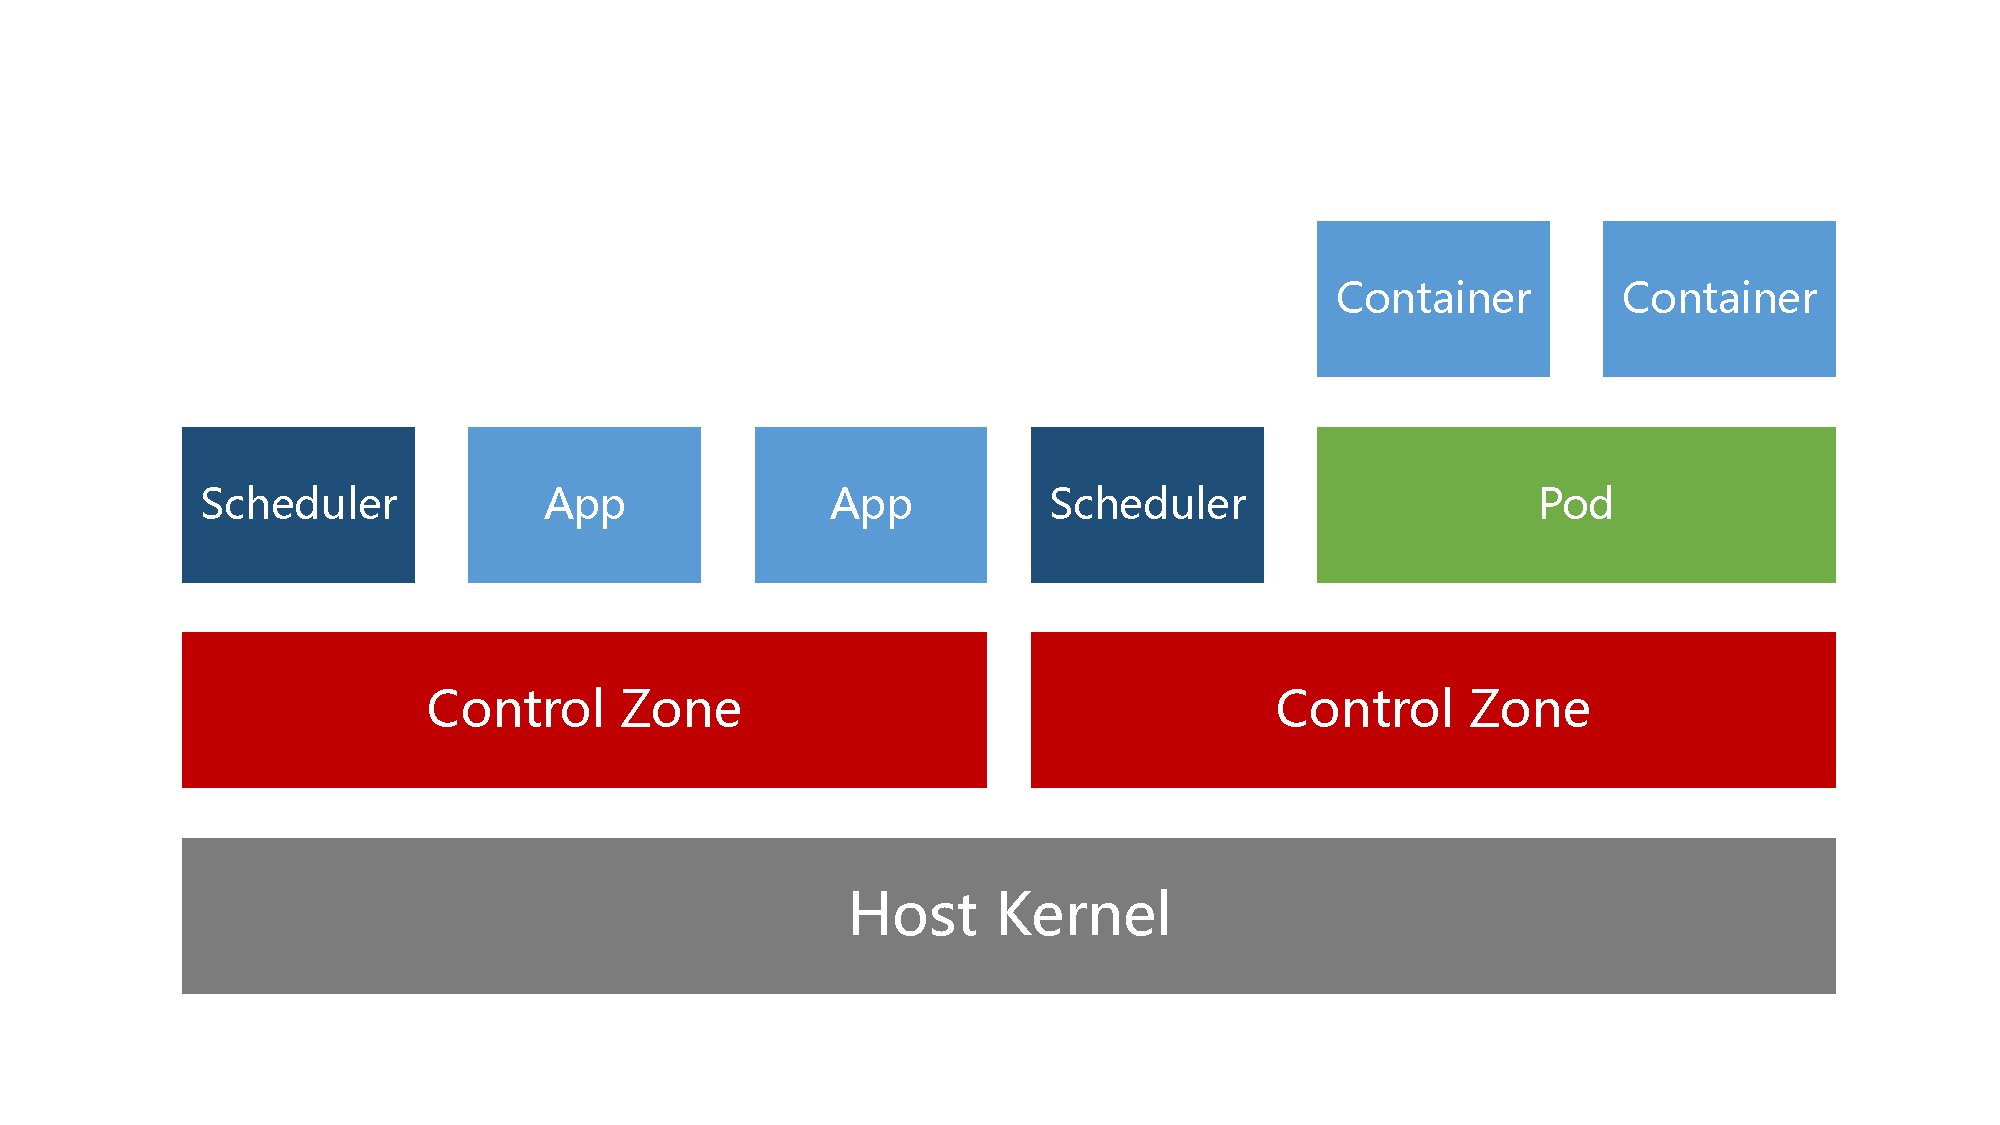
\includegraphics[width=0.7\textwidth]{controlzone}
    \bicaption{\quad Control Zone架构}{\quad Control Zone Architectural}
    \label{fig:controlzone}
\end{figure}

\section{本章小结}